\chapter{Implementierung}

\section{Einleitung}

Ziel dieser Arbeit war es, eine Simulationsumgebung für Sensorknoten zu schaffen. Es sollte viele verschiedene Arten von Sensorknoten geben, die jeweils einen oder mehrere verschiedene Sensoren besitzen. Mit diesen Knoten sollte ein Netzwerk aufgebaut werden, um die Umgebungsparameter eines Gebietes zu erfassen.
Die Daten der Simulation sollten visualisiert und ausgewertet werden.

\section{Aufbau und Struktur}

\subsection{Klassenübersicht}

Die Klassenübersichten wurden teilweise mit Hilfe von doxygen\cite{doxygen} erstellt. 

\begin{figure}[htbp]
\centering
\caption{Klassenübersicht}
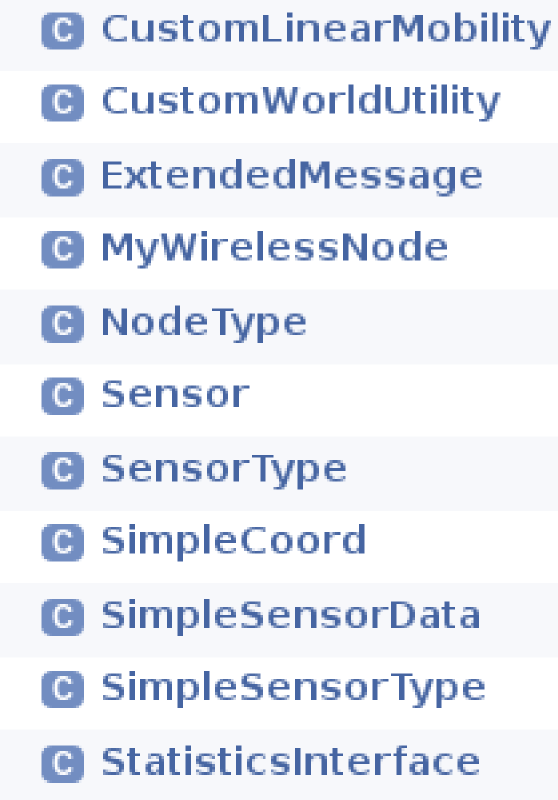
\includegraphics{Klassenuebersicht}
\end{figure}

\subsubsection{CustomLinearMobility}

\begin{figure}[htbp]
\centering
\caption{CustomLinearMobility: Vererbung}
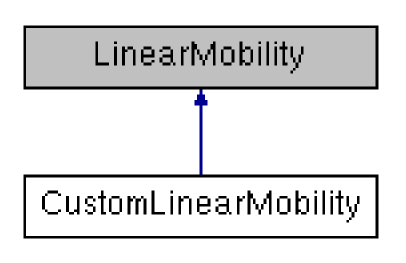
\includegraphics{CustomLinearMobility}
\end{figure}

Diese Klasse erbt direkt von der in MiXiM definierten LinearMobility. Sie ist um einige Parameter erweitert, die es ermöglichen, dass die Knoten beschleunigen können und eine maximale Geschwindigkeit \textbf{maxSpeed} erreichen, sollte eine definiert sein.
Der Parameter \textbf{maxSpeed} kann ebenso auf 0 gesetzt werden, um die Knoten von mobil in stationär umzuwandeln.

\subsubsection{CustomWorldUtility}

Die Klasse CustomWorldUtility ist eine der wichtigsten für die Simulation. Sie repräsentiert den \textbf{Playground}, also den Bereich indem sich die Knoten befinden. Sie erbt von der Klasse BaseWorldUtility aus dem MiXiM-Framework. BaseWorldUtility stellt die nötigen Funktionalitäten für den Playground bereit. \newline

\begin{figure}[htbp]
\centering
\caption{CustomWorldUtility: Vererbung}
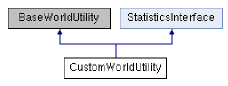
\includegraphics{CustomWorldUtility1}
\end{figure}

Zusätzlich dazu stellt die Klasse selbst die notwendigen Parameter für die Umwelt bereit. Nach dem Starten der Simulation steht darin jeweils ein zweidimensionales Array pro Sensortyp bereit: temperatureArray, pressureArray, humidityArray und lightArray. Diese enthalten die Parameter der Umgebung; temperatureArray beinhaltet zum Beispiel, wie der Name schon sagt, Informationen über die Temperatur. \newline
Es kann zu Beginn der Simulation entschieden werden, ob neue Werte berechnet werden sollen oder die bereits vorhandenen Werte für die Umgebung übernommen werden sollen. Die Arrays besitzen die gleiche Größe wie der Playground. Diese Größe ist auch zusätzlich in den Parametern sizeX und sizeY gespeichert.


\begin{figure}[htbp]
\centering
\caption{CustomWorldUtility: Member}
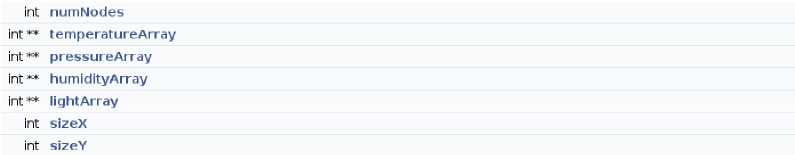
\includegraphics[width=\textwidth]{CustomWorldUtility3}
\end{figure}

Zum Erstellen neuer Daten kann die Funktion \textbf{generateEnvironmentData()} genutzt werden. Es ist dadurch auch möglich während der Simulation neue Werte zu generieren, indem man diese Funktion aufruft. Die Funktion legt pro Umweltparameter eine xml-Datei im Ordner \textit{WorldModel/data} an. Jede der xml-Dateien wird beim Start mit Hilfe der Funktion \textbf{readXML(int)} eingelesen, verarbeitet, also in ein Array umgewandelt und anschließend in der Klasse gespeichert. \newline
Sollte nun ein Sensor nach dem Wert an seiner aktuellen Position fragen, so kann diese Klasse mit Hilfe der Funktionen \textbf{generateMessage(const char*)} und \textbf{sendSensorResponse(std::string, cGate *)} eine Antwort generieren. Die Position kann dabei mit der Klasse \textbf{SimpleCoord} und der Wert an dieser Position mit \textbf{SimpleSensorData} repräsentiert und per Nachricht verschickt werden.

\begin{figure}[htbp]
\centering
\caption{CustomWorldUtility: Methoden}
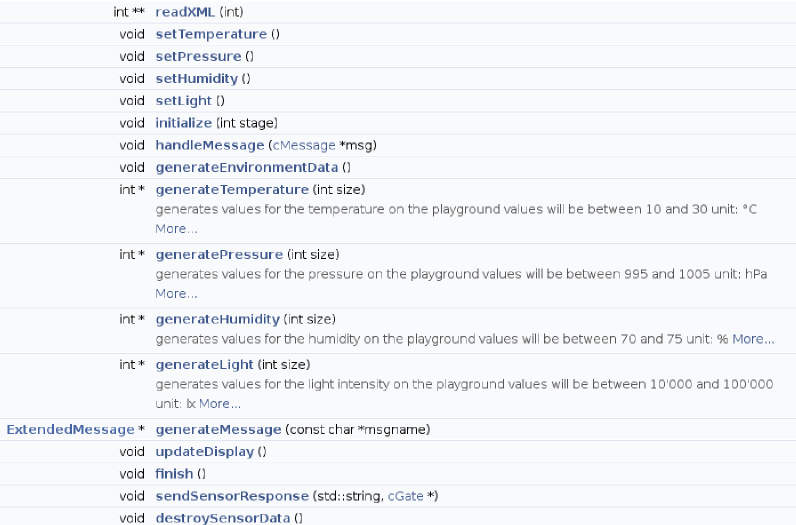
\includegraphics[width=\textwidth]{CustomWorldUtility2}
\end{figure}

\paragraph{Einblick in einige Funktionen}

Wie im vorigen Abschnitt beschrieben übernimmt die Funktion generateEnvironmentData() das Erstellen von Umweltparametern. Dafür ruft sie, je nach Sensordatentyp, eine der folgenden Funktionen auf:

\begin{multicols}{2}
\begin{itemize}
\item generateTemperature() - $^\circ $C
\item generatePressure() - hPa
\item generateHumidity()- \%
\item generateLight() - lx
\end{itemize}
\end{multicols}

Diese Funktionen generieren ein 2-dimensionales Array in der Größe des Playgrounds mit Werten, die die jeweils oben angegebenen Einheiten besitzen. In Listing \ref{lst:generateTemp} ist die generateTemperature()-Funktion als ein Beispiel aufgeführt. Im Falle dieser Funktion werden Zufällige integer-Werte generiert, welche sich im Bereich 10 bis 30 bewegen.

\begin{lstlisting}[language=C++, label=lst:generateTemp]
int* CustomWorldUtility::generateTemperature(int size)
{
    int* data = new int[size];
    for (int i = 0; i < size; i++) {
        //10 - 30
        data[i] = (int)((rand() % 100)/5) + 10;
    }
    return data;
}
\end{lstlisting}

Um eben diese Daten wieder lesen zu können dient die Funktion readXML(). Sie verwendet die cXMLElement-Funktionen aus dem Omnet++-Framework. Diese ist sehr hilfreich beim Verarbeiten von XML-Dateien. Da in dieser Simulation die Umweltparameter in Form von XML gespeichert sind, ist dies eine sehr nützliche Funktionalität.

\begin{lstlisting}[language=C++]
int** CustomWorldUtility::readXML(int fileName)
{
    // get the xml from the parameter, return type cXMLElement
    [...]

    // get a vector (of type cXMLElement) with all childs of the root-tag
    cXMLElementList nListRows = rootE->getChildren();
    int amountRows = nListRows.size();

    int** data = new int*[amountRows];
    for (int i = 0; i < amountRows; i++){
        //this is a row as cXMLElement
        cXMLElement* nListRowArray = nListRows[i];
        //this is a list of an entire row as cXMLElements
        cXMLElementList nLeafElementsList = nListRowArray->getChildren();
        int amountColumns = nLeafElementsList.size();
        data[i] = new int[amountColumns];
        for (int j = 0; j < amountColumns; j++) {
            data[i][j] = atoi(nLeafElementsList[i]->getNodeValue());
        }
    }

    return data;
}
\end{lstlisting}

Die bis jetzt beschriebenen Funktionen werden alle bereits bei der Initialisierung der Simulation ausgeführt. Während der Laufzeit sind dagegen Andere von Bedeutung. Die zentrale Funktion für die Kommunikation ist hier, wie auch bei anderen Klassen, die handleMessage(cMessage)-Funktion. \newline
Diese wartet auf eine Nachricht vom Typ 'GET [Sensortyp]'. Sollte eine solche Nachricht ankommen, so ist diese vom Typ ExtendedMessage, kommt von einem Sensor und enthält einen Parameter, welcher die Position des anfragenden Sensors beinhaltet. Mit diesen Informationen wird die Funktion sendSensorResponse aufgerufen.

\begin{lstlisting}[language=C++]
void CustomWorldUtility::sendSensorResponse(string sensorType, cGate* srcGate, SimpleCoord* position)
{
    SimpleSensorData *data;
    if (sensorType == "temperature") {
        data = new SimpleSensorData("data", this->temperatureArray[(int)position->x][(int)position->y]);
    } else if (sensorType == "pressure") {
        data = new SimpleSensorData("data", this->pressureArray[(int)position->x][(int)position->y]);
    } else if (sensorType == "humidity") {
        data = new SimpleSensorData("data", this->humidityArray[(int)position->x][(int)position->y]);
    } else if (sensorType == "light") {
        data = new SimpleSensorData("data", this->lightArray[(int)position->x][(int)position->y]);
    } else {
        throw new exception;
    }

    string messageName = "POST ";
    messageName += sensorType;
    ExtendedMessage *newmsg = generateMessage(messageName.c_str());
    newmsg->getParList().add(data);
    string gateName = srcGate->getBaseName();
    gateName += "$o";
    int index = srcGate->getIndex();
    send(newmsg, gateName.c_str(), index);//"worldDataGate$o"
    numSent++;
}
\end{lstlisting}

Diese erzeugt eine Antwort auf den GET-Request. Mit Hilfe des Sensortypes und der Position auf dem Playground wird das korrekte Parameterarray und die x- und y-Koordinate bestimmt und der darin stehende Integer-Wert als SimpleSensorData gespeichert.
Diese neu erzeugt Instanz wird anschließend an eine Nachricht der Form 'POST [Sensortyp]' angehängt und an den Sender zurück geschickt.

\subsubsection{MyWirelessNode und Sensor}

MyWirelessNode implementiert das StatisticsInterface und erbt von der Klasse Sensor, welche vom cSimpleModule erbt. Die Klasse Sensor soll lediglich mehr Struktur in die Klasse MyWirelessNode bringen und die Funktionen und Attribute in jene unterteilen, welche für die allgemeine Kommunikation und weiteres verantwortlich sind und jene, die nur für die Sensordaten zuständig sind. \newline

\begin{figure}[htbp]
\centering
\caption{MyWirelessNode: Vererbung}
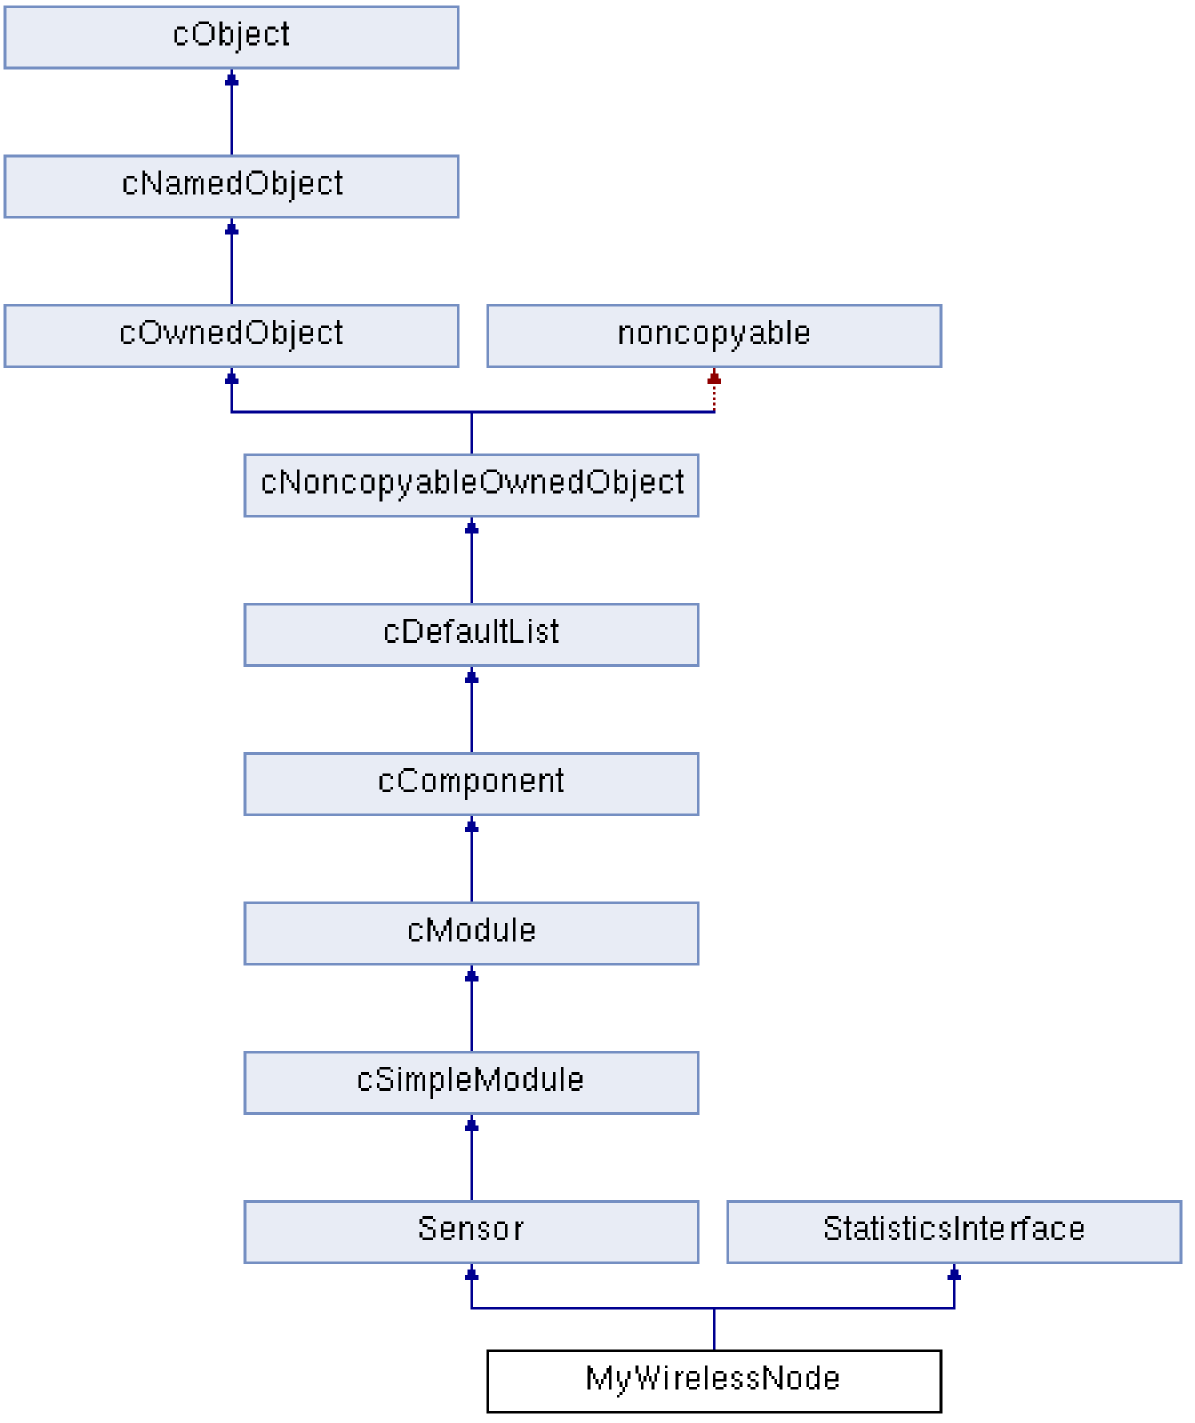
\includegraphics{MyWirelessNode}
\end{figure}

Es ist neben der Klasse für die Umwelt CustomWorldUtility die zweite essentielle Klasse der Simulation. Das Verhalten aller Knoten im Netzwerk wird durch MyWirelessNode definiert. Neben den Standardfunktionen eines Omnet++-Moduls, \textbf{initialize()}, \textbf{handleMessage()} und \textbf{finish()}, können Knoten zum Beispiel ihre Position abfragen. \newline
Dazu dient die Funktion \textbf{updatePosition()} \ref{lst:updatePosition}, welche das Attribut \textbf{position} aktualisiert.

\begin{minipage}{\textwidth}
\begin{lstlisting}[language=C++, label=lst:updatePosition]
/**
 * update the position data by a given Coord object
 */
void MyWirelessNode::updatePosition()
{
    Coord* back;
    BasePhyLayer* phy = FindModule<BasePhyLayer*>::findSubModule(this);
    ChannelMobilityPtrType pMobType = phy->getMobilityModule();
    if(pMobType != NULL){
        back = new Coord(pMobType->getCurrentPosition());
        delete position;
        position = back;
    }
}
\end{lstlisting}
\end{minipage}
Dafür wird die Klasse FindModule aus dem MiXiM-Framework verwendet. Diese enthält eine Funktion findSubModule(cModule), welche zum Finden von service-ähnlichen Modulen dient. Die FindModule-Klasse verhält sich für diese Art von Klassen, wie eine Art Servicemanager.\newline
Auf diese Weise hat man Zugriff auf das Mobility-Modul eines bestimmten Sensorknotens und kann aus diesem die aktuelle Position auf dem Playground abrufen.\newline
Des weiteren beinhaltet das Modul MyWirelessNode Funktionen zum Anfordern von Umweltdaten. Dies erfolgt über einen GET request an das World-Modul, welches anschließend eine Antwort darauf sendet. Dafür stehen die Funktionen requestData() und sendDataRequest(std::string)\ref{lst:requestData} zur Verfügung, wobei sendDataRequest(std::string) innerhalb von requestData() aufgerufen wird.
\begin{lstlisting}[language=C++, label=lst:requestData]
void MyWirelessNode::requestData()
{
    updatePosition();

    //generate messages for data requests
    std::string request = "GET ";
    if (this->type->humidity) {
        this->sendDataRequest(request + this->typenames[0]);
    }
    if (this->type->pressure) {
        this->sendDataRequest(request + this->typenames[1]);
    }
    if (this->type->temperature) {
        this->sendDataRequest(request + this->typenames[2]);
    }
    if (this->type->light) {
        this->sendDataRequest(request + this->typenames[3]);
    }
}

void MyWirelessNode::sendDataRequest(std::string request)
{
    ExtendedMessage *newmsg = generateMessage(request.c_str());
    SimpleCoord *coord = new SimpleCoord("pos", this->position);
    newmsg->getParList().add(coord);
    std::stringstream s;
    s << "X: " << coord->x << " Y: " << coord->y;
    ev.bubble(this, s.str().c_str());
    send(newmsg, "toWorld$o");
    numSent++;
}
\end{lstlisting}

Um aktuelle Daten anfordern zu können wird zunächst immer die aktuell gespeicherte Position des Knoten aktualisiert. Danach wird zu jedem Sensortyp des Knotens eine Nachricht vom Typ 'GET [Sensortyp]' erstellt, mit den aktuellen Koordinaten bestückt und anschließen an die CustomWorldUtility gesendet.

\subsubsection{NodeType}

NodeType erbt von der Klasse cModuleType und erfüllt den gleichen Zweck. Es ist dazu da die MyWirelessNode-Klassen für jeden Knoten anzulegen, sodass diese global bekannt sind, verwendet werden können und am Ende der Simulation wieder gelöscht werden.

\begin{figure}[htbp]
\centering
\caption{NodeType: Vererbung}
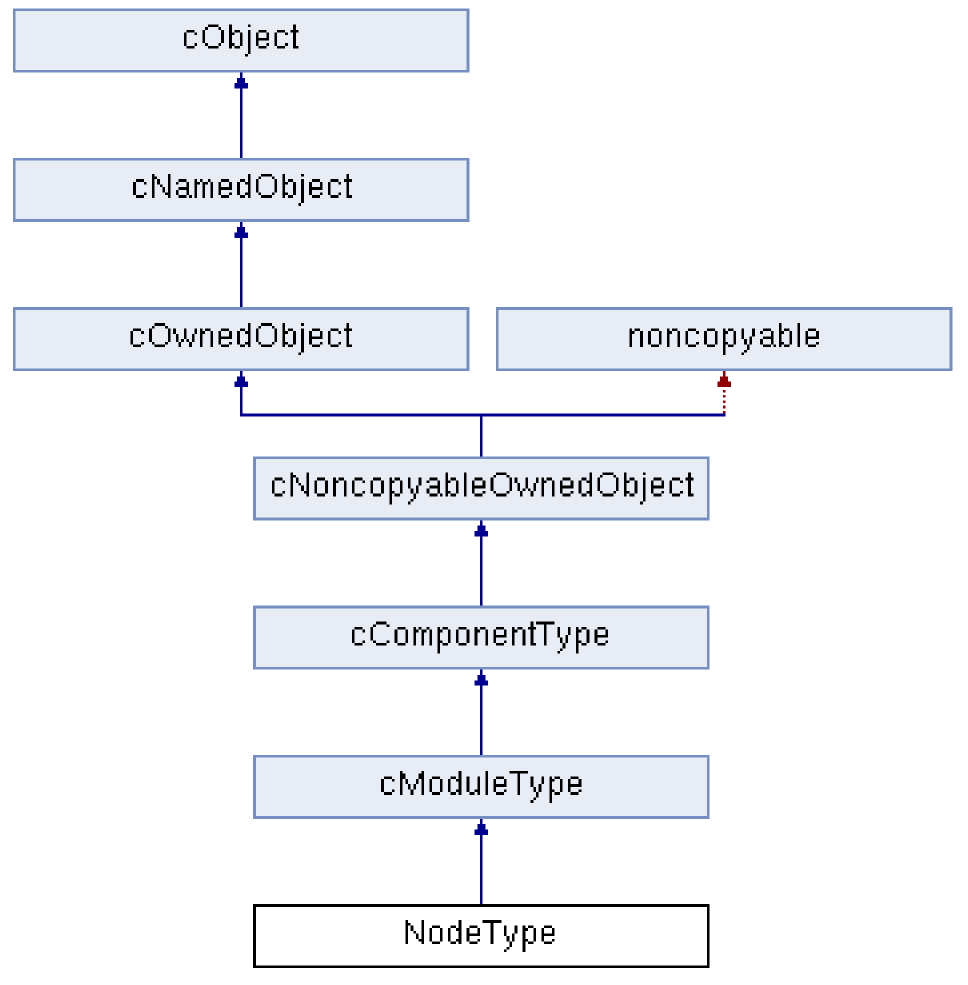
\includegraphics{NodeType}
\end{figure}

\subsubsection{SensorType}

\begin{figure}[htbp]
\centering
\caption{SensorType: Member}
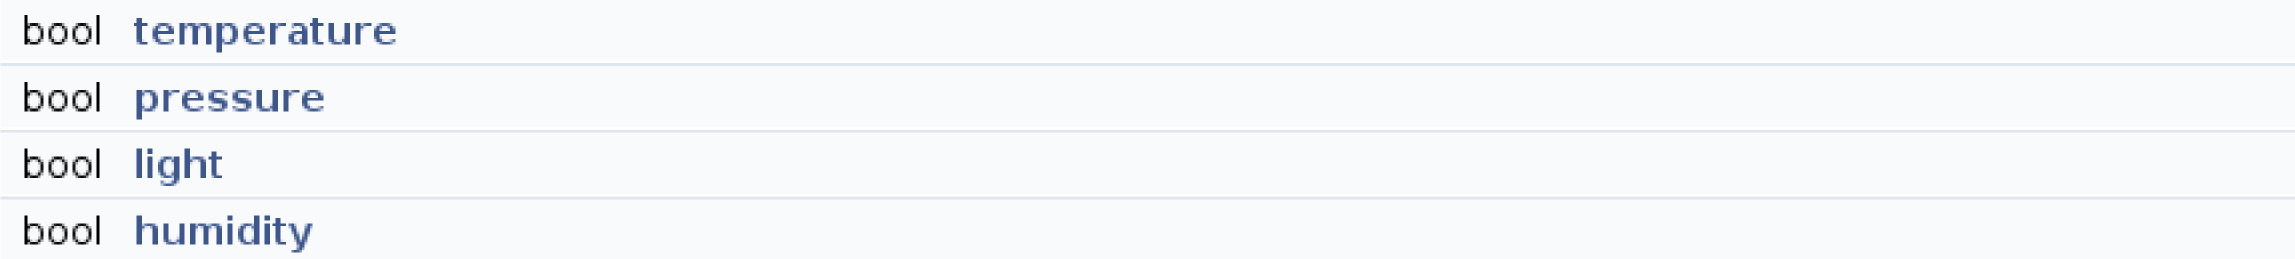
\includegraphics[width=\textwidth]{SensorType}
\end{figure}

Die Klasse SensorType ist eine Helferklasse für MyWirelessNode. Es besitzt lediglich 4 Attribute, welche definieren ob der jeweilige Knoten einen bestimmten Typ von Sensor besitzt oder nicht.

\subsubsection{Simple*}

\begin{figure}[htbp]
\centering
\caption{SimpleClasses: Member}
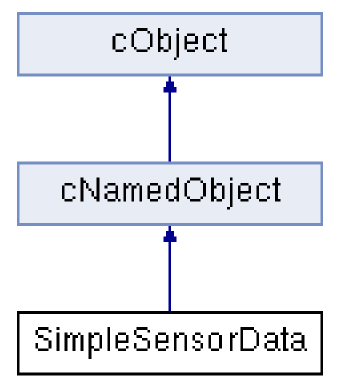
\includegraphics{SimpleClasses}
\end{figure}

Es gibt die 3 Klassen SimpleCoord, SimpleSensorData und SimpleSensorType.  Sie erben jeweils direkt von cNamedObject und beinhalten nur wenige Attribute. So enthält SimpleCoord beispielsweise 3 Attribute x, y und z, um Koordinaten zu repräsentieren.\newline
cNamedObject und ebenso Kinderklassen davon lassen sich per leicht cMessage übertragen. Alle haben daher den Zweck eine einfache Kommunikation zu ermöglichen. So wird beispielsweise SimpleCoord benutzt, um beim Anfordern von Sensordaten in MyWirelessNode die Koordinaten an die CustomWorldUtility mit zu übertragen, damit in der Response der jeweilige Datensatz der richtigen Position zurückgegeben wird.\newline
Aus diesem Grund ist die einzig benutzte Funktion in diesen Modulen der Konstruktor. Beim Erstellen einer der Klassen werden die nötigen Variablen gesetzt und an die Instanz ein Name vergeben. So lassen sich diese Objekte nach dem Hinzufügen zur Parameterliste einer Klasse auch leicht wieder abrufen (siehe Bespiel \ref{lst:SimpleExample}).

\begin{lstlisting}[language=C++, label=lst:SimpleExample]
//im Sender:
cMessage *msg = new cMessage(msgname);
SimpleCoord *coord = new SimpleCoord("position", this->position);
msg->getParList().add(coord);

//
// Nachricht uebertragen    
//  
  
//im Empfaenger:  
SimpleCoord *position = (SimpleCoord*) msg->getParList().remove("position");
\end{lstlisting}

\subsubsection{ExtendedMessage}

ExtendedMessage erbt direkt von der Klasse cMessage, der Standard-Nachrichtenklasse in Omnet++. Im Grunde stellt cMessage alle benötigten Funktionen bereit. ExtendedMessage ist nur aus dem Grund vorhanden, um zusätzliche Statistiken über Nachrichten erstellen zu können, zum Beispiel wie oft eine einzelne Nachricht weitergesendet wurde.

\begin{figure}[htbp]
\centering
\caption{ExtendedMessage: Vererbung}
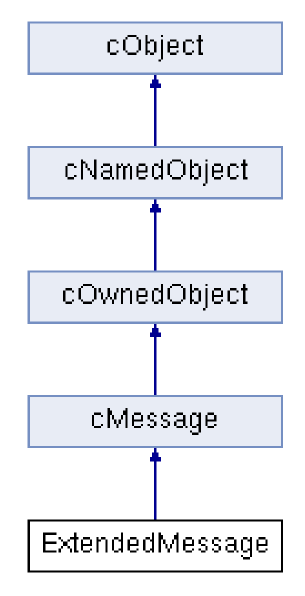
\includegraphics{ExtendedMessage}
\end{figure}

Im Listing \ref{lst:ExtendedMessage} ist zu sehen welche Statistikparameter erhoben werden.

\begin{minipage}{\textwidth}
\begin{lstlisting}[language=NED, label=lst:ExtendedMessage]
message ExtendedMessage extends cMessage
{
	int source;
    int destination;
    int hopCount = 0;    
}
\end{lstlisting}
\end{minipage}
\subsubsection{StatisticsInterface}

Dieses Interface enthält grundlegende Attribute für Statistiken. Klassen die dieses implementieren speichern somit zum Beispiel wie viele Nachrichten sie empfangen oder gesendet haben.


\subsection{Übersicht NED-Module}

Im folgenden Abschnitt werden alle Simulationsobjekte erläutert, also all jene, die durch die Sprache NED beschrieben wurden:

\begin{itemize}{\label{enum:Netzwerk}}
\item Simple Module
\begin{multicols}{2}
\begin{itemize}
\item CustomLinearMobility
\item CustomWorldUtility  
\item HumiditySensor
\item LightSensor
\item PressureSensor
\item Sensor
\item TemperatureSensor 
\end{itemize}
\end{multicols}
\item Compound Module
\begin{multicols}{2}
\begin{itemize}
\item HLNode
\item HLPNode
\item HNode
\item HPNode
\item LNode
\item LPNode
\item MyWirelessNode
\item PNode
\item THLNode
\item THLPNode
\item THNode
\item THPNode
\item TLNode
\item TLPNode
\item TNode
\item TPNode 
\end{itemize}
\end{multicols}
\begin{multicols}{2}
\item Networks
\begin{itemize}
\item MyNetwork
\end{itemize}
\item Messages
\begin{itemize}
\item ExtendedMessage
\end{itemize}
\end{multicols}
\end{itemize}

\subsubsection{Simple Module}

Simple Module sind Komponenten in einer Omnet++ Simulation, die die größte Auswirkung auf die Wirkungsweise des Netzwerkes haben. Das liegt daran, dass bei ihnen neben einer Beschreibung in NED auch eine Beschreibung in C++ vorliegt. Daher kann das Verhalten jener Module während der Simulation ausführlich definiert werden.

\paragraph{CustomLinearMobility}

Das Modul CustomLinearMobility ist eine Erweiterung der LinearMobility, welche MiXiM bereitstellt. Neben dem Verhalten welches in C++ beschrieben ist, ist das Modul lediglich um den Parameter maxSpeed erweitert, welcher in der omnetpp.ini definiert werden kann.

\paragraph{CustomWorldUtility}

Wie im Codebeispiel (\ref{lst:CustomWorldUtility}) zu sehen ist, ist das Modul CustomWorldUtility eine Erweiterung des Moduls BaseWorldUtility. Zusätzlich zu den darin definierten Eigenschaften hat es einige weitere Parameter. Zunächst eine bool'sche Variable, welche festlegt, ob zu Beginn der Simulation neue Umweltparameter generiert werden sollen. \newline Während numSensorNodes definiert, wieviele Sensorknoten im Netzwerk vorhanden sind und somit wieviele Gates zu Sensorknoten gehen, so definiert numGates die Anzahl der einzelnen Sensoren und somit auch die Anzahl der dahin gehenden notwendigen Gates. Da Sensorknoten auch mit mehr als einem Sensor bestückt sein können, ist der Wert beider Variablen mitunter durchaus verschieden.\newline
Die restlichen Variablen speichern die Umweltparameter in Form einer xml-Datei.

\begin{minipage}{\textwidth}
\begin{lstlisting}[language=ned,caption={CustomWorldUtility},label=lst:CustomWorldUtility]
package mynetwork.WorldModel;
import org.mixim.base.modules.BaseWorldUtility;

simple CustomWorldUtility extends BaseWorldUtility
{
    parameters:
        bool createData;
        int numGates;
        int numSensorNodes;
        xml xmlTemperature = xmldoc("WorldModel/data/temperature.xml");
        xml xmlPressure = xmldoc("WorldModel/data/pressure.xml");
        xml xmlHumidity = xmldoc("WorldModel/data/humidity.xml");
        xml xmlLight = xmldoc("WorldModel/data/light.xml");
        
        @class("CustomWorldUtility");
    gates:
        inout worldDataGate[numGates];
        inout toNode[numSensorNodes];
}
\end{lstlisting}
\end{minipage}

Neben den Parametern besitzt dieses Modul auch noch zusätzlich 2 verschiedene Arten von inout-Gates. Die Menge von worldDataGates verbindet die Welt mit jedem Sensor der auf einem Sensorknoten verbaut ist. Die Menge der toNode-Gates dient für die direkte Verbindung zwischen World und Nodes.

\paragraph{Sensoren}

Es gibt 5 Module welche die Sensoren definieren. Zum einen den allgemeinen Sensor, der das Vatermodul für alle 4 Sensortypen bildet. Er enthält nicht viel, lediglich Gates für Verbindungen zur Welt, um die Umweltparameter abfragen zu können und zum jeweiligen Knoten, für die Kommunikation innerhalb des Bauteils. Weiterhin besitzt er noch einen Parameter, der im Kindmodul den Typ des Sensors beschreibt.

\begin{multicols}{2}
\begin{itemize}
\item HumiditySensor
\item LightSensor
\item PressureSensor
\item TemperatureSensor
\end{itemize}
\end{multicols}

Die 4 Sensortypen, welche vom allgemeinen Sensor erben, definieren jeweils nur den Typ des Sensors. Sie können auf den Knoten als Submodule verwendet werden. Jeder Sensorknoten kann 1 bis 4 Sensoren verschiedener Typen beinhalten und somit ergeben sich 15 verschiedene Arten von Sensorknoten.

\begin{minipage}{\textwidth}
\begin{lstlisting}[language=ned,caption={Sensor},label=lst:Sensor]
package mynetwork.Node.Sensor;

simple Sensor 
{
    parameters:
        //type of the sensor
        string type;
	    @display("i=block/wrx");
	    @class("Sensor");
	gates: 
	    inout toNode;
	    inout worldDataGate;
}
\end{lstlisting}
\end{minipage}

\subsubsection{Compound Module}

Compound Module dienen dazu, andere Module zusammenzufassen, sollen jedoch keine eigene aktive Funktionalität definieren. Ihr Verhalten soll sich allein durch die Submodule ergeben. Es ist daher nicht sinnvoll eine C++-Klasse für diese Module zu definieren.\newline
Alle Sensorknoten, die in dieser Simulation vorkommen sind solche Compound Module.

\paragraph{MyWirelessNode}

Zum einen existiert das Modul MyWirelessNode, welches das Vatermodul für alle Sensorknoten bildet. Es erbt selbst von einem Modul, welches die kabellose Kommunikation unter den Knoten und Batteriestatistiken ermöglicht. Außerdem beinhalten die Knoten auch Funktionen der Mobility, genauer gesagt der CustomLinearMobility, welche auch mobile Knoten ermöglicht. \newline
Es besitzt weiterhin ein inout Gate zur World.

\paragraph{Sensorknoten}

Es gibt insgesamt 15 verschiedene Arten von Sensorknoten, welche am Anfang von Kapitel \ref{enum:Netzwerk} aufgelistet sind. Die Benennung ergibt sich wie folgt (jeweils aus dem Anfangsbuchstaben des englischen Begriffs):
\begin{itemize}
\item T - Temperatur
\item H - Luftfeuchtigkeit
\item L - Licht
\item P - Druck
\end{itemize}
Hierzu ein Codebeispiel des NED-Modules des Knotens, der alle 4 Sensoren enthält: Listing \ref{lst:THLPNode}.

\begin{lstlisting}[language=ned,caption={THLPNode},label=lst:THLPNode]
package mynetwork.Node;
import mynetwork.Node.Sensor.TemperatureSensor;
import mynetwork.Node.Sensor.HumiditySensor;
import mynetwork.Node.Sensor.LightSensor;
import mynetwork.Node.Sensor.PressureSensor;

module THLPNode extends MyWirelessNode
{
    @display("bgb=210,491");
    gates:
        inout toSensor[4];
        inout worldGate[4];

    submodules:
        TemperatureSensor: TemperatureSensor {
            @display("p=140,380");
        }
        HumiditySensor: HumiditySensor {
            @display("p=140,310");
        }
        LightSensor: LightSensor {
            @display("p=140,450");
        }
        PressureSensor: PressureSensor {
            @display("p=70,450");
        }

    connections:
        toSensor[0] <--> { delay = 0ms; } <--> TemperatureSensor.toNode;
        worldGate[0] <--> { delay = measureTime; } <--> TemperatureSensor.worldDataGate;

        toSensor[1] <--> { delay = 0ms; } <--> HumiditySensor.toNode;
        worldGate[1] <--> { delay = measureTime; } <--> HumiditySensor.worldDataGate;
        
        toSensor[2] <--> { delay = 0ms; } <--> LightSensor.toNode;
        worldGate[2] <--> { delay = measureTime; } <--> LightSensor.worldDataGate;
        
        toSensor[3] <--> { delay = 0ms; } <--> PressureSensor.toNode;
        worldGate[3] <--> { delay = measureTime; } <--> PressureSensor.worldDataGate;
}
\end{lstlisting}

Wie man sehen kann erbt der Sensorknoten von MyWirelessNode. Er übernimmt zunächst also alle Eigenschaften des vorher bereits erklärten Modules. Hinzu kommen pro Sensor jeweils 1 Gate zum Sensor und zur world, welches den Sensor mit der Welt verbindet. \newline
Entscheidend für das jeweilige Modul ist jedoch die Definition der Submodule. Im Falle des THLPNode werden genau 4 Submodule definiert:
\begin{itemize}
\item TemperatureSensor
\item HumiditySensor
\item LightSensor
\item PressureSensor
\end{itemize}
Also für jeden Sensor das jeweilige Modul.\newline
Zuletzt werden noch für die Gates die Verbindungen definiert.

\subsubsection{Networks}

Das Netzwerk ist das wichtigste Modul jeder Omnet++-Simulation, denn es fügt alle Elemente zusammen. Ein Netzwerk ist den Compound-Modulen daher nicht unähnlich. 

\paragraph{MyNetwork}

Für das Modul MyNetwork heißt das, dass es eine Instanz des CustomWorldUtility und variabel viele Sensorknoten zusammenfügt, indem es diese als Submodule definiert und deren Gates miteinandern verbindet. Die Definition ist dem MiXiM-Modul BaseNetwork ähnlich, aber hat deutlich mehr zusätzliche Submodule und Parameter. \newline
So sind die Definitionen des Playgrounds, der Mobilität und des ConnectionManager analog, die Submodule der World und des Sensorknoten und die dazu benötigten Parameter, die zum Beispiel die Anzahl der jeweiligen Sensorknoten definieren und die Gateverbindungen jedoch kommen nur hier vor.

\begin{lstlisting}[language=ned,caption={Network},label=lst:Network]
network MyNetwork
{
    parameters:
        bool createNewEnvironmentData;

        //...

        int numTNodes = default(0);
        //...
        int numTHLPNodes = default(0);

        // total number of hosts in the network
        int numNodes = numTNodes + numPNodes + numHNodes + numLNodes + numTHNodes + numTLNodes + numTPNodes + numHLNodes + numHPNodes + numLPNodes + numTHLNodes + numTLPNodes + numTHPNodes + numHLPNodes + numTHLPNodes;
        string wuType = default("CustomWorldUtility");

        //BaseNetwork
        double playgroundSizeX @unit(m); // x size of the area the nodes are in (in meters)
        double playgroundSizeY @unit(m); // y size of the area the nodes are in (in meters)
        double playgroundSizeZ @unit(m); // z size of the area the nodes are in (in meters)
        **.mobility.constraintAreaMinX = default(0m);
        **.mobility.constraintAreaMinY = default(0m);
        **.mobility.constraintAreaMinZ = default(0m);
        **.mobility.constraintAreaMaxX = default(playgroundSizeX);
        **.mobility.constraintAreaMaxY = default(playgroundSizeY);
        **.mobility.constraintAreaMaxZ = default(playgroundSizeZ);
        string cmType = default("org.mixim.base.connectionManager.ConnectionManager"); // connection manager to use

        @display("bgi=maps/germany,bgb,$playgroundSizeX,$playgroundSizeY,white;bgp=0,0;bgb=$playgroundSizeX,$playgroundSizeY");

    submodules:
        world: CustomWorldUtility {
            //for every sensor (NOT only every node) there is one gate needed
            numGates = numNodes 
            + numTHNodes + numTLNodes + numTPNodes + numHLNodes + numHPNodes + numLPNodes 
            + 2*numTHLNodes + 2*numTLPNodes + 2*numTHPNodes + 2*numHLPNodes 
            + 3*numTHLPNodes;
            numSensorNodes = numNodes;
            createData = createNewEnvironmentData;
        }
        
        tnode[numTNodes]: TNode {
            parameters:
                @display("i=device/card");
                numHosts = numNodes;
        }
        //...
        thlpnode[numTHLPNodes]: THLPNode {
            parameters:
                @display("i=device/card");
                numHosts = numNodes;
        }

        connectionManager: <cmType> like IConnectionManager {
            parameters:
                @display("i=abstract/multicast;is=s");
        }


    connections allowunconnected:

        world.worldDataGate++ 
        <--> {  delay = 100ms; } <--> 
        tnode[i].worldGate[0] for i=0..(numTNodes-1);		
        //...		
        world.worldDataGate++ 
        <--> {  delay = 100ms; } <--> 
        thlpnode[i].worldGate[3] for i=0..((numTHLPNodes-1));

        world.toNode++ 
        <--> {  delay = 0ms; } <--> 
        tnode[i].toWorld for i=0..(numTNodes-1);
        //...
        world.toNode++ 
        <--> {  delay = 0ms; } <--> 
        thlpnode[i].toWorld for i=0..(numTHLPNodes-1);
}
\end{lstlisting}

Nicht auf den ersten Blick zu erkennen ist die Kommunikation zwischen den Knoten selbst. Die connections sind durch den Term allowunconnected so definiert, dass auch dynamisch Verbindungen aufgebaut werden können, die nicht strikt im Compound Module  definiert sind. Mit Hilfe der sendDirect()-Funktion können so dennoch Nachrichten zwischen Gates versendet werden.

\subsubsection{Messages}

Nachrichten sind das essentielle Werkzeug, um in einem Netzwerk Kommunikation zu ermöglichen. Es gibt ein vordefiniertes Modul cMessage, welches dafür genutzt werden kann. Dieses beinhaltet notwendige Informationen wie zum Beispiel Sendermodul und -gate, Empängermodul und -gate, Sende-, Empfangs- und Erstellzeit und mehr.

\paragraph{ExtendedMessage}

Die ExtendedMessage erweitert diese Funktionalität um einige Informationen für die Statistik.

\begin{lstlisting}[language=ned,caption={ExtendedMessage},label=lst:ExtendedMessage]
message ExtendedMessage extends cMessage
{
    int source;
    int destination;
    int hopCount = 0;    
}
\end{lstlisting}

\subsubsection{omnetpp.ini}

Die omnetpp.ini ist eine Datei, in der Eigenschaften der Simulation geändert werden können, ohne das man den Sourcecode bearbeiten und danach neu kompilieren muss. Es bietet sich daher an, alle Variablen und Konstanten, welche sich öfters ändern hier zu definieren.\newline

\begin{lstlisting}
##########################################################
#    		   Custom Parameters	                     #
##########################################################

#informations
##set maxspeed to 0mps for stationary nodes or to any higher value for mobility nodes
**.mobility.maxSpeed = 0mps
#**.mobility.maxSpeed = 10mps

#this boolean value defines if new data for the sensor will be created
MyNetwork.createNewEnvironmentData = ask

#set the amount of nodes here
MyNetwork.howManyHumidityAndTemperatureNodes = ask
[...]

#set the number of nodes for the simulation here
#MyNetwork.numNodes = 1
MyNetwork.networkPosX = 0
MyNetwork.networkPosY = 0
MyNetwork.networkSensorAlgorithm = 1
MyNetwork.networkValue = -1
**.netwl.headerLength = 24bit

#**.mobilityType = "CustomLinearMobility" -> NED default
#Gaussian distribution for the acceleration with a mean of 1 leads to a result if ~half of the nodes will end stationary
**.mobility.speed = 1mps
**.mobility.acceleration = normal(1, 1)
**.mobility.angle = default

#Playground
**.playgroundSizeX = 400m
**.playgroundSizeY = 550m
\end{lstlisting}

Für die relevanten Parameter wurde in der ini-Datei eine spezielle Sektion eingeteilt. Hier können beispielsweise Werte für die playgroundSize vergeben oder festgelegt werden ob Mobilität der Knoten erlaubt sein soll.

\section{Funktionsweise}

All die in diesem Kapitel beschriebenen Module wirken für die Simulation zusammen, um ein Netzwerk aus Sensorknoten zu schaffen, in dem die Knoten miteinander und mit ihrer Umgebung gemeinsam agieren können. Dazu werden nach dem Start der Simulation Umweltparameter bereitgestellt und eine festgelegte Anzahl von verschiedenen Sensorknoten erzeugt. Diese können sich anschließend bewegen oder ihr Position beibehalten. Sie können mit ihren Sensoren Werte der Umgebung erfassen und diese über Funk an andere Sensorknoten übertragen, sollte diese in der näheren Umgebung zur Verfügung stehen.

\begin{figure}[htbp]
\centering
\caption{Verlauf der Nachrichten und Methodenaufrufe}
\includegraphics[width=\textwidth]{Nachrichtenverlauf}
\end{figure}